\FILE{usage.tex}

\section{FutureGrid Usage}

When offering services such as FutureGrid to the community, we have to
analyse and predict which services may be useful for the users. We
have therefore established a number of activities that monitor
external and interanl data. Externally, we look for example at
information provided by Gartners technology hype curve \cite{?} or
Google trend information as shown in Figure \ref{F:google-trend}. From
Google Trend data we observe that the populariity of Grid computing
has been very low  in the recent years and much attention has shifted
to cloud computing. Therefore we removed this information from the
figure and focuss exemplary on cloud related terms such as {\em Cloud
  Computing}, {\em Big Data}, {\em OpenStack} {\em VMWare}.
From this information we see that all but VMWare are rising, with
Cloud Computing dominating the google trends in comparision to the
others. This trend is important as it shows a shift in the cloud
computing community buzz away from a traditional commecial market
leader in virtualization technology. We believe that is correlated
with a large number of vendors offering alternative prducts and
services while at the same time the novelty from VMWare is reduced.

\begin{figure}[htb]
 \centering
    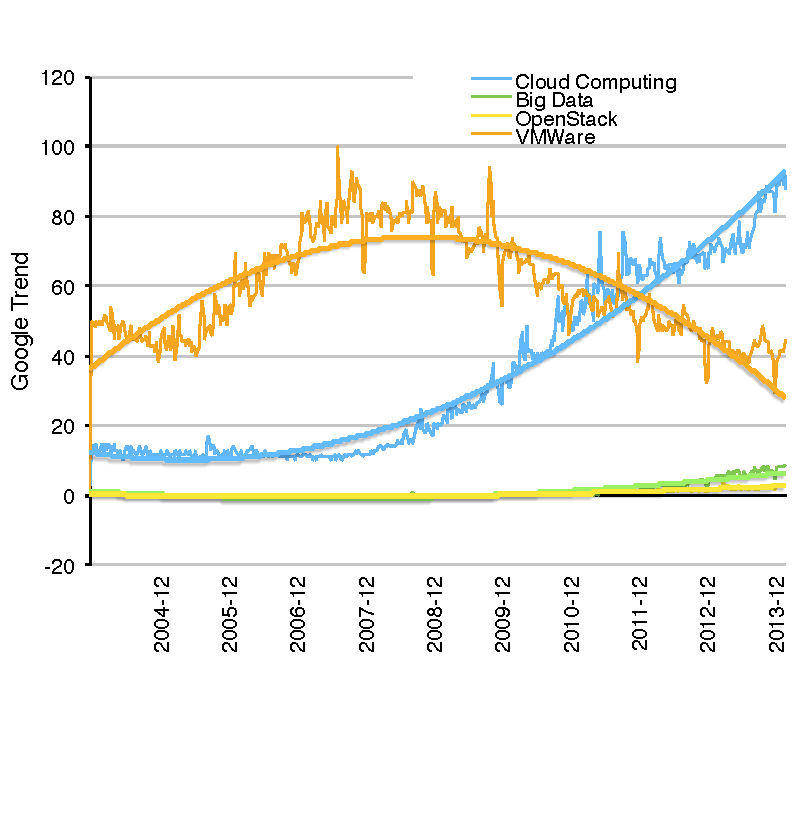
\includegraphics[width=.75\textwidth]{images/google-trend.pdf}
  \caption{Google Trends.}\label{F:google-trend}
\end{figure}

To give an informal overview of the more than 300 projects conducted
on FutureGrid we have taken their titles and display them in a word
cloud (see Figure \ref{F:wordcloud}. Additionally, we have taken
keywords that are provided by the project leades and also displayed
the in a word cloud (see Figure \ref{F:keycloud}. Although the
imagesdoe not give quantitative perspective about the project it helps
to identify some rough idea about the activities that are ongoing in FutureGrid.
As expected the terms cloud computing an and terms such as mapreduce,
Openstack, Nimbus, and Eucalyptus appear quite frequently. It is hence
worthwhile to analyse this data in a more quantitative form.

\begin{figure}[htb]
\begin{minipage}[t]{0.5\textwidth}
  \centering
    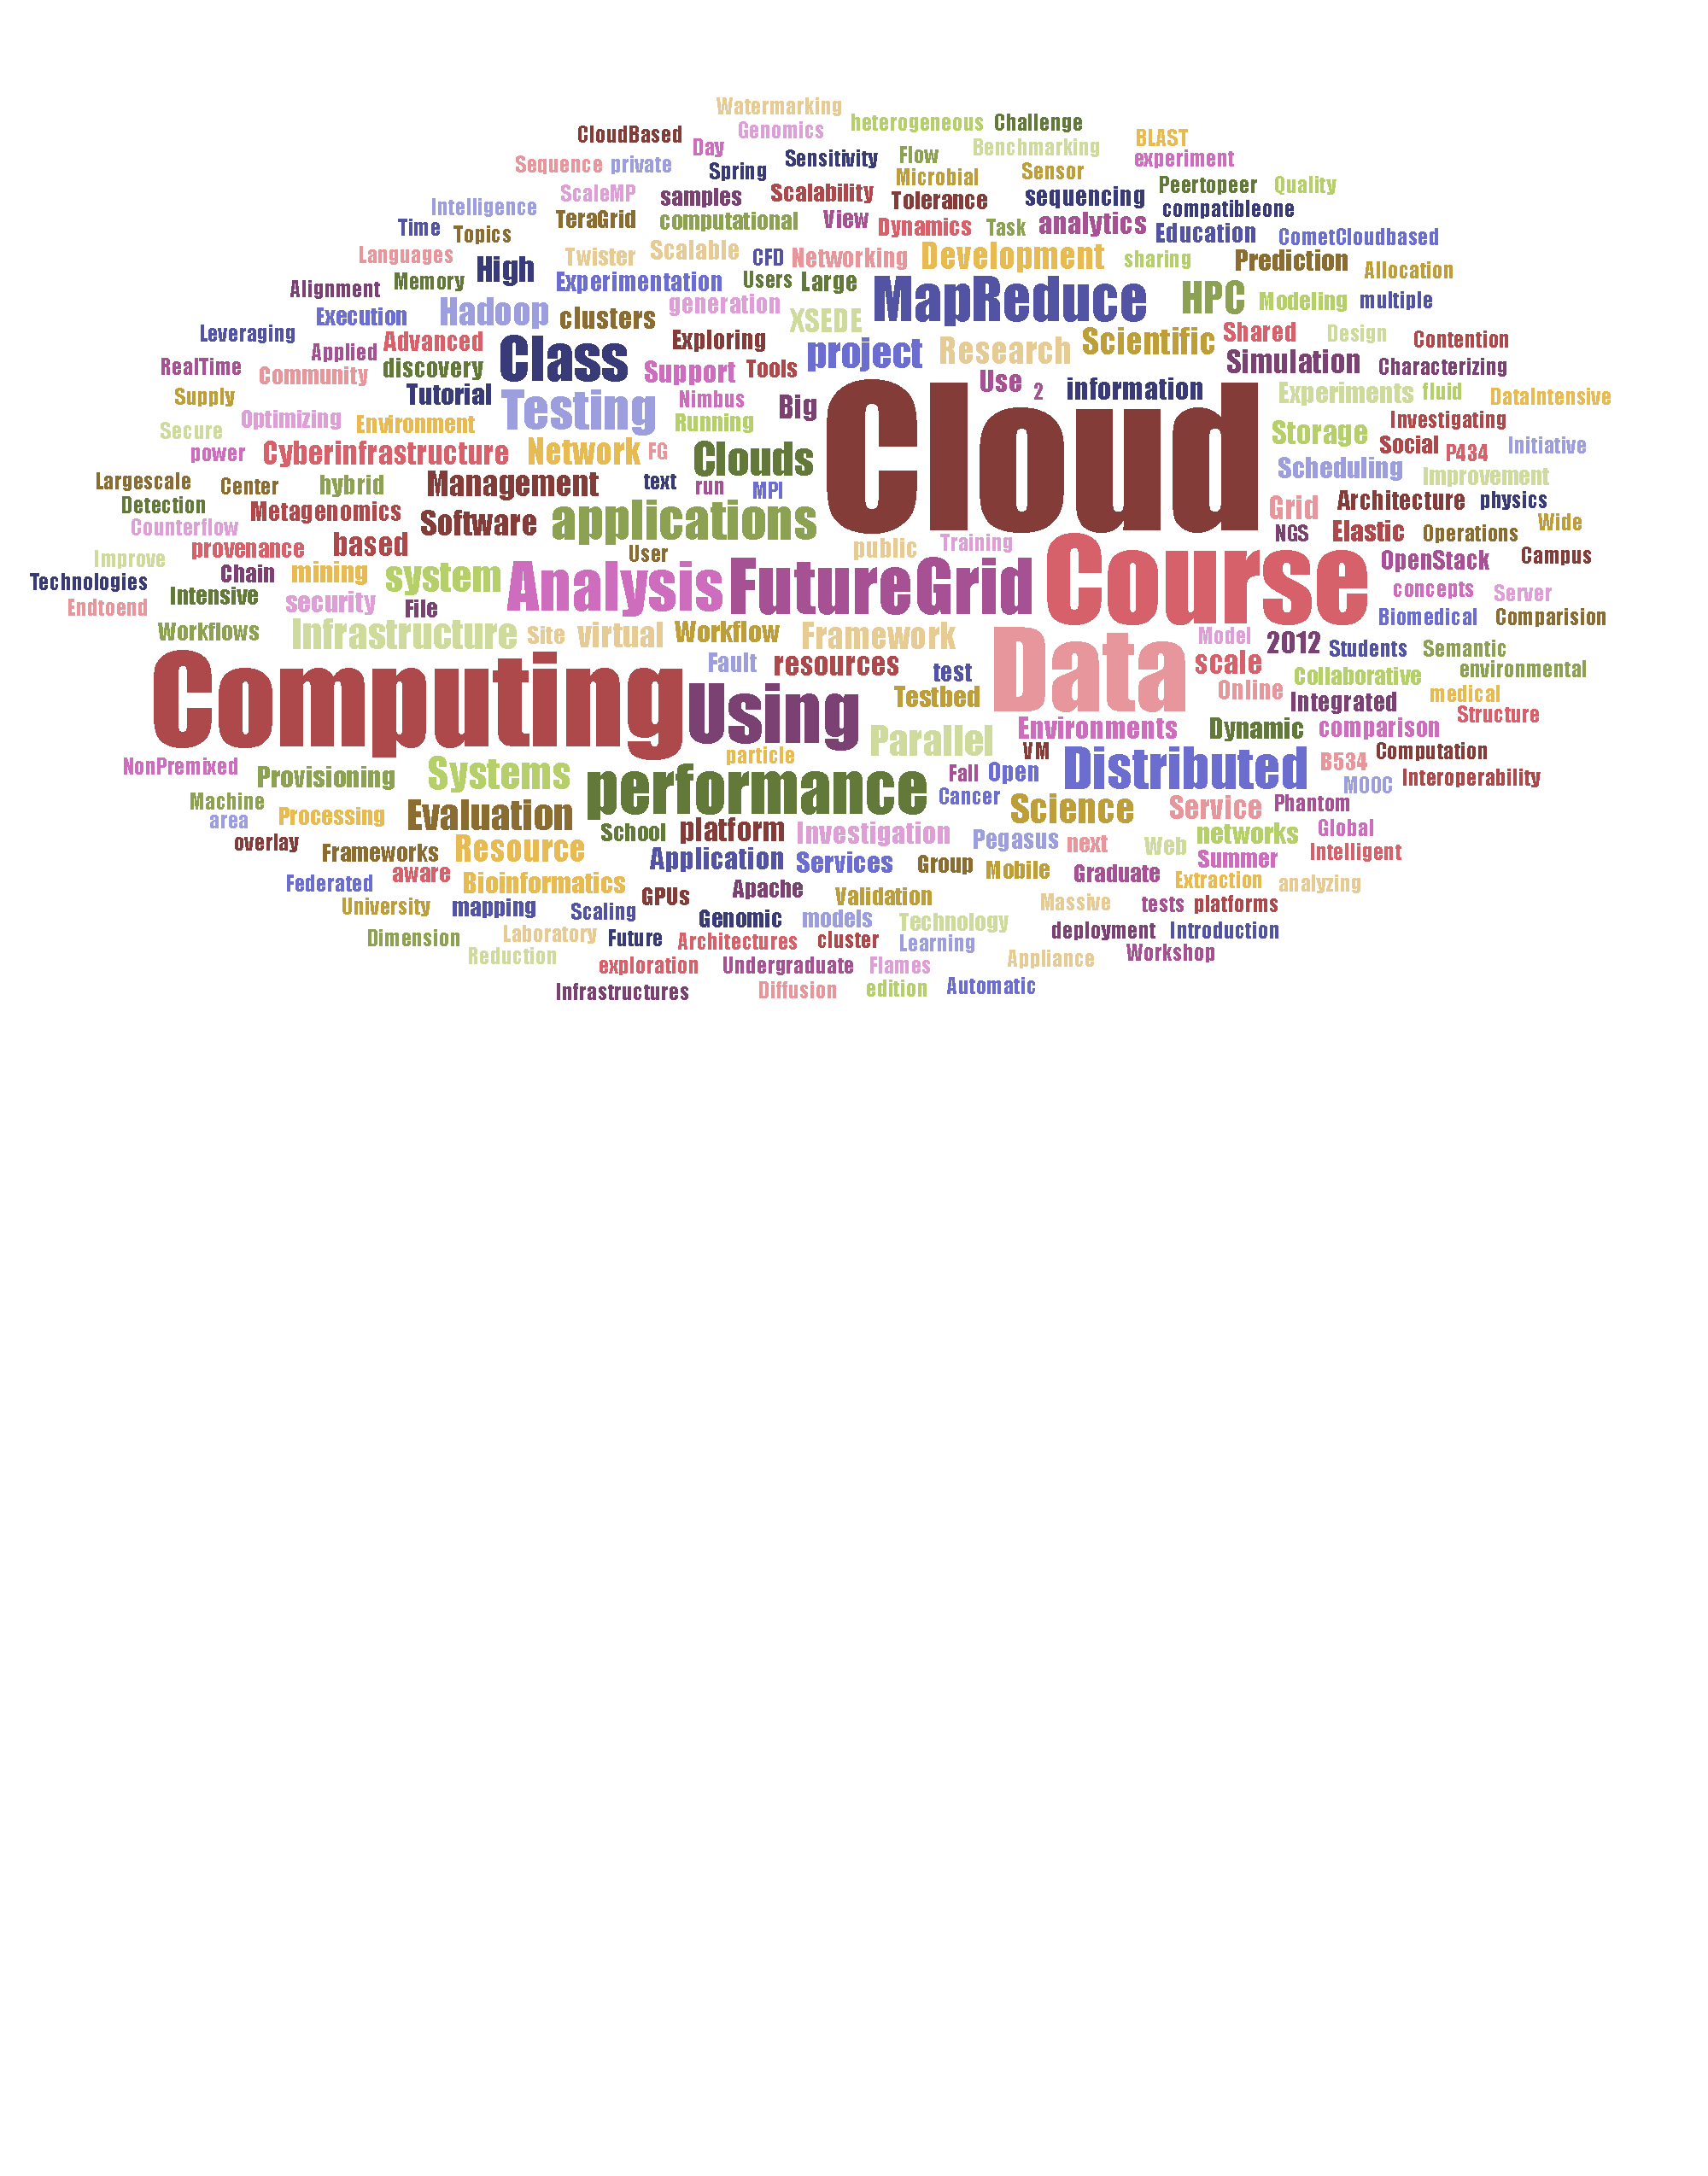
\includegraphics[width=1.0\textwidth]{images/fg-title-wordcloud.pdf}
  \caption{Project title word cloud.}\label{F:wordcloud}
\end{minipage}
\begin{minipage}[t]{0.5\textwidth}
  \centering
    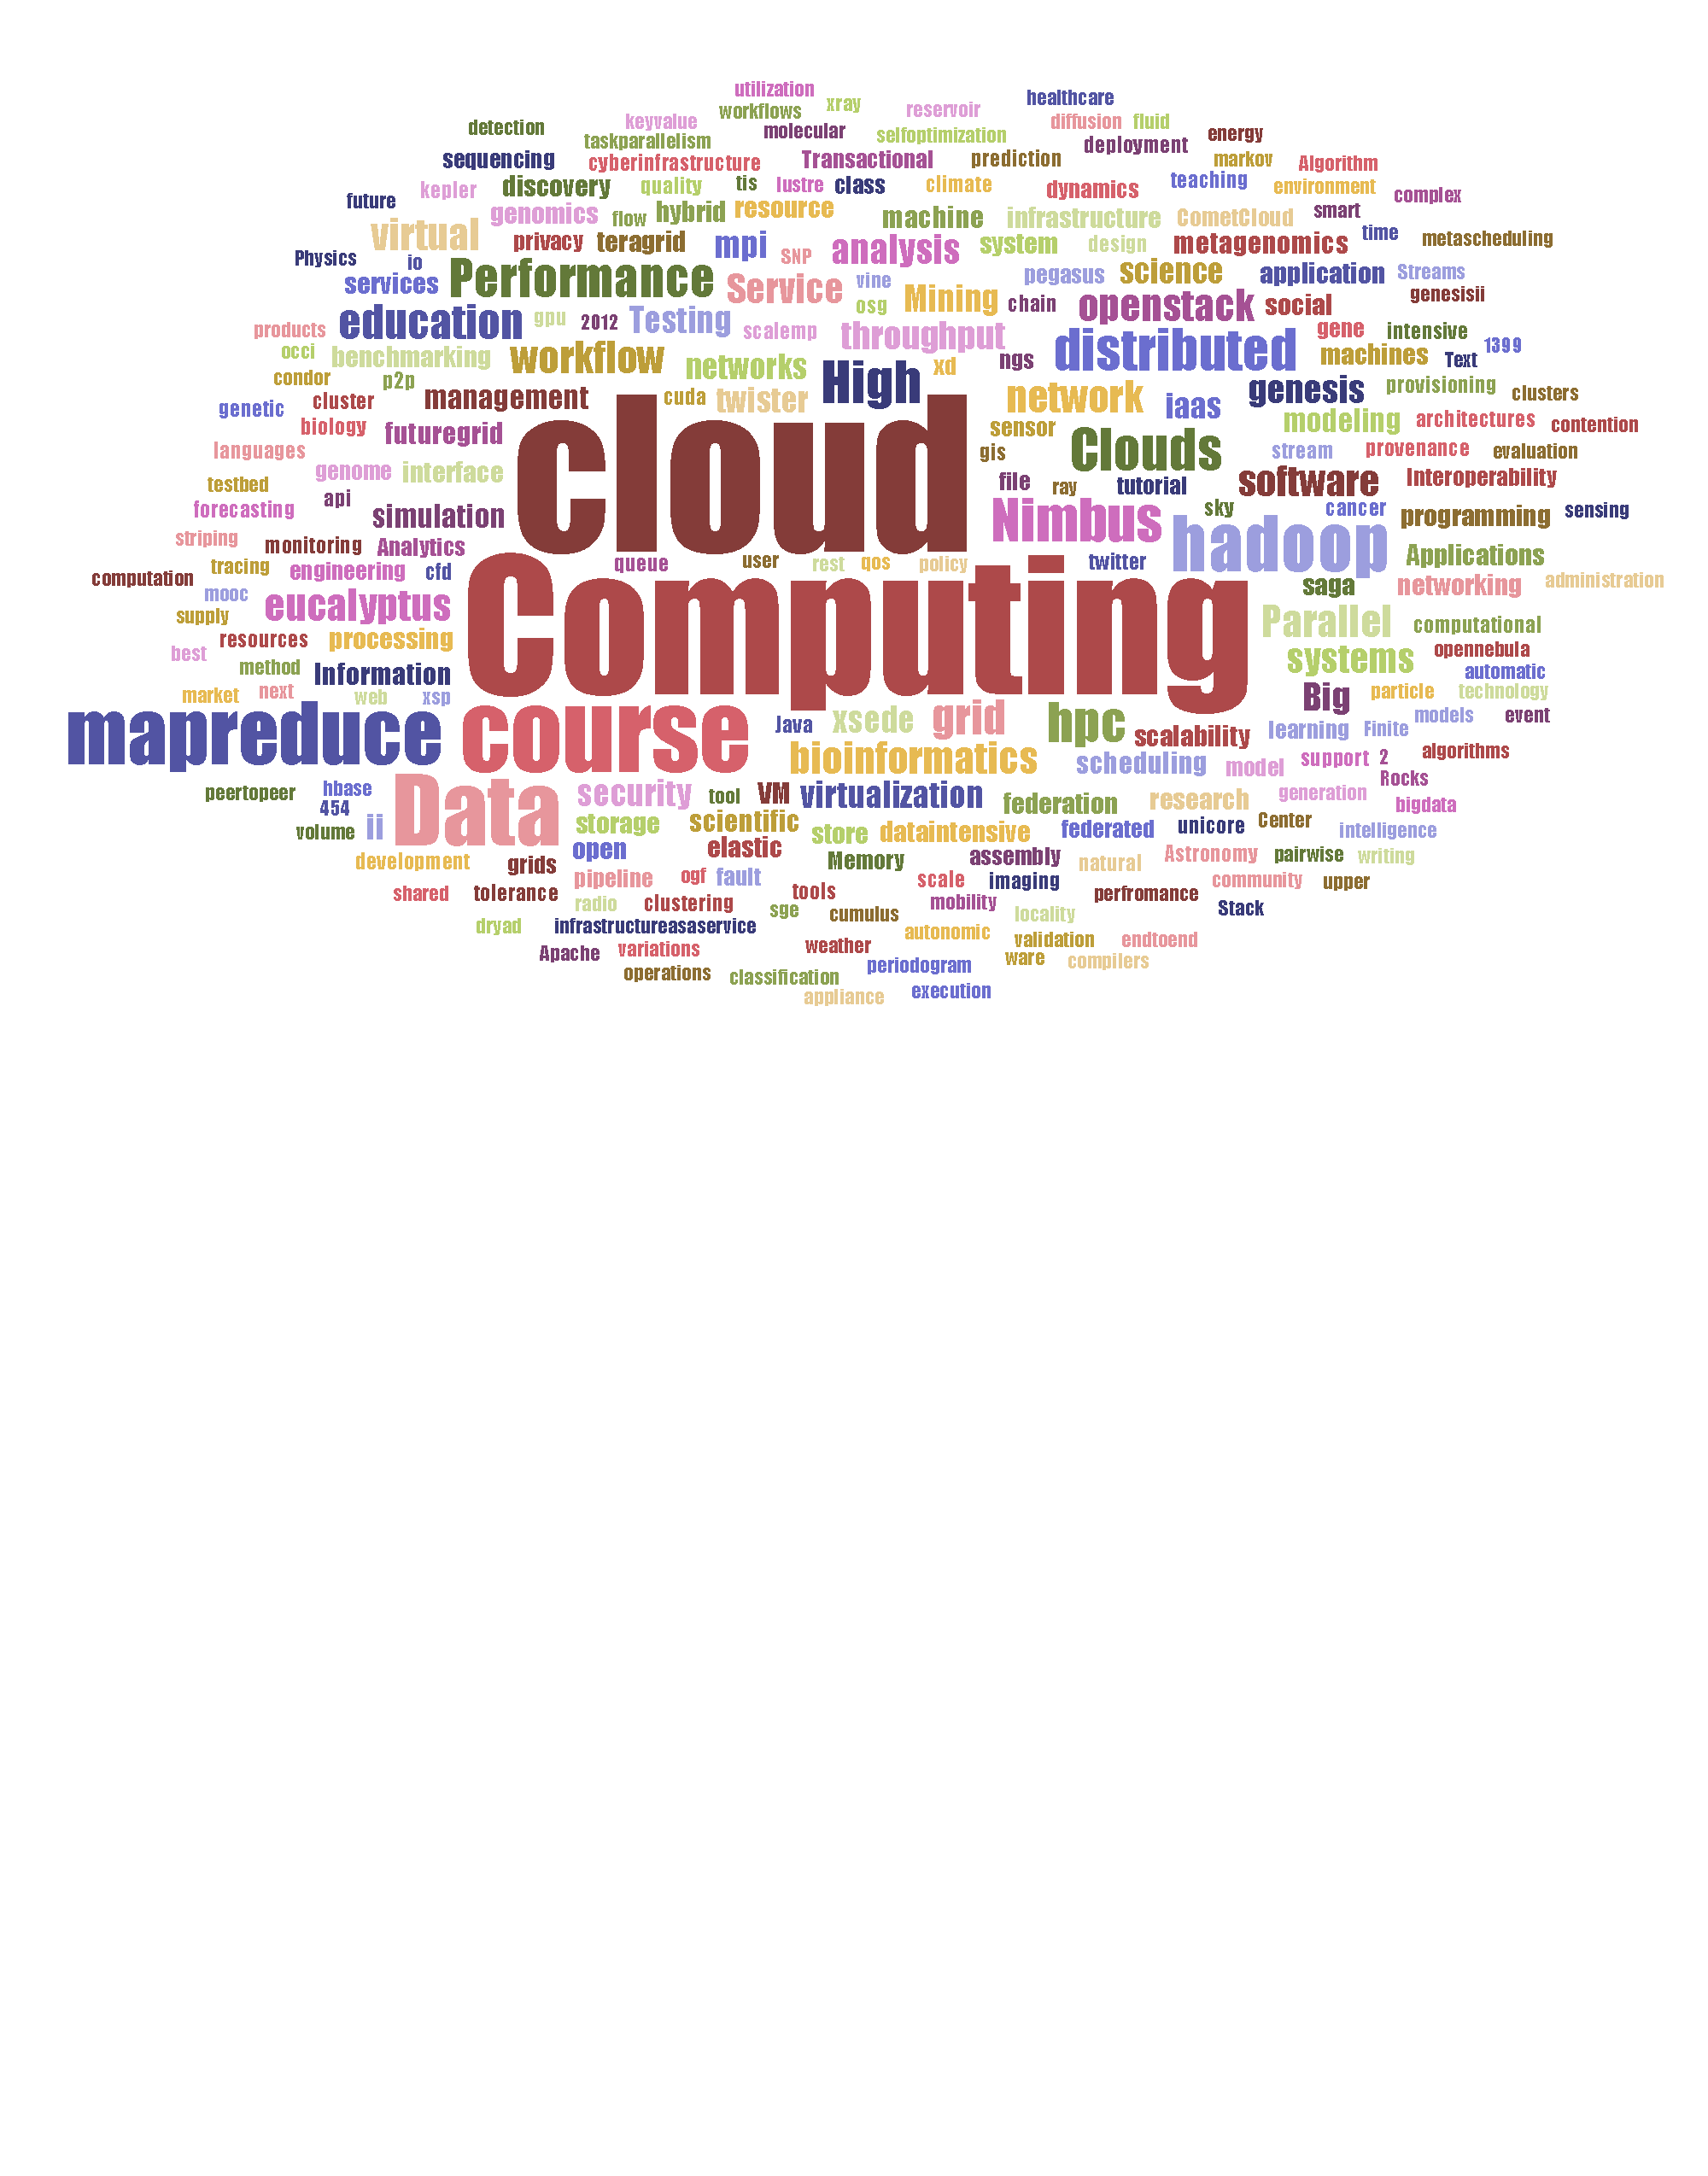
\includegraphics[width=1.0\textwidth]{images/fg-keyword-wordcloud.pdf}
  \caption{Project keyword word cloud.}\label{F:keycloud}
\end{minipage}
\end{figure}


As part of our project management in FutureGird we have designed a
simple project application procedure that includes prior to a project
granted access gathering information about which technologies are
anticipated to be used within the project. The list is fairly
extensive and includes Grid, HPC, and Cloud computing systems,
services, and software. However, for this paper we will focus
primerally on technologies that are dominantly requested and depicted
in Figure~\ref{F:request-tech}. Clearly we can identify the trend,
that shows the increased popularity of OpenStack within the services
offered on FutureGrid. Nimbus and Eucalyptus are on a significant
downwards trend. ObenNebula was also at one point more reqested that
either Nimbus or Eucalyptus, but do to limited manpower an official
version of OpenNebula was not made available. As we have not offered
it and pointed it out on our Web page, requests for OpenNebula have vanished.
However internally have used OpenNebula for projects such as our cloudmesh rain
framework. All other sixteen technologies are relatively equally
distributed over the monitoring period. The lesson that we took form
this is that FutureGrid has put more emphasize in offereing OpenStack Services.

\begin{figure}[htb]
  \centering
    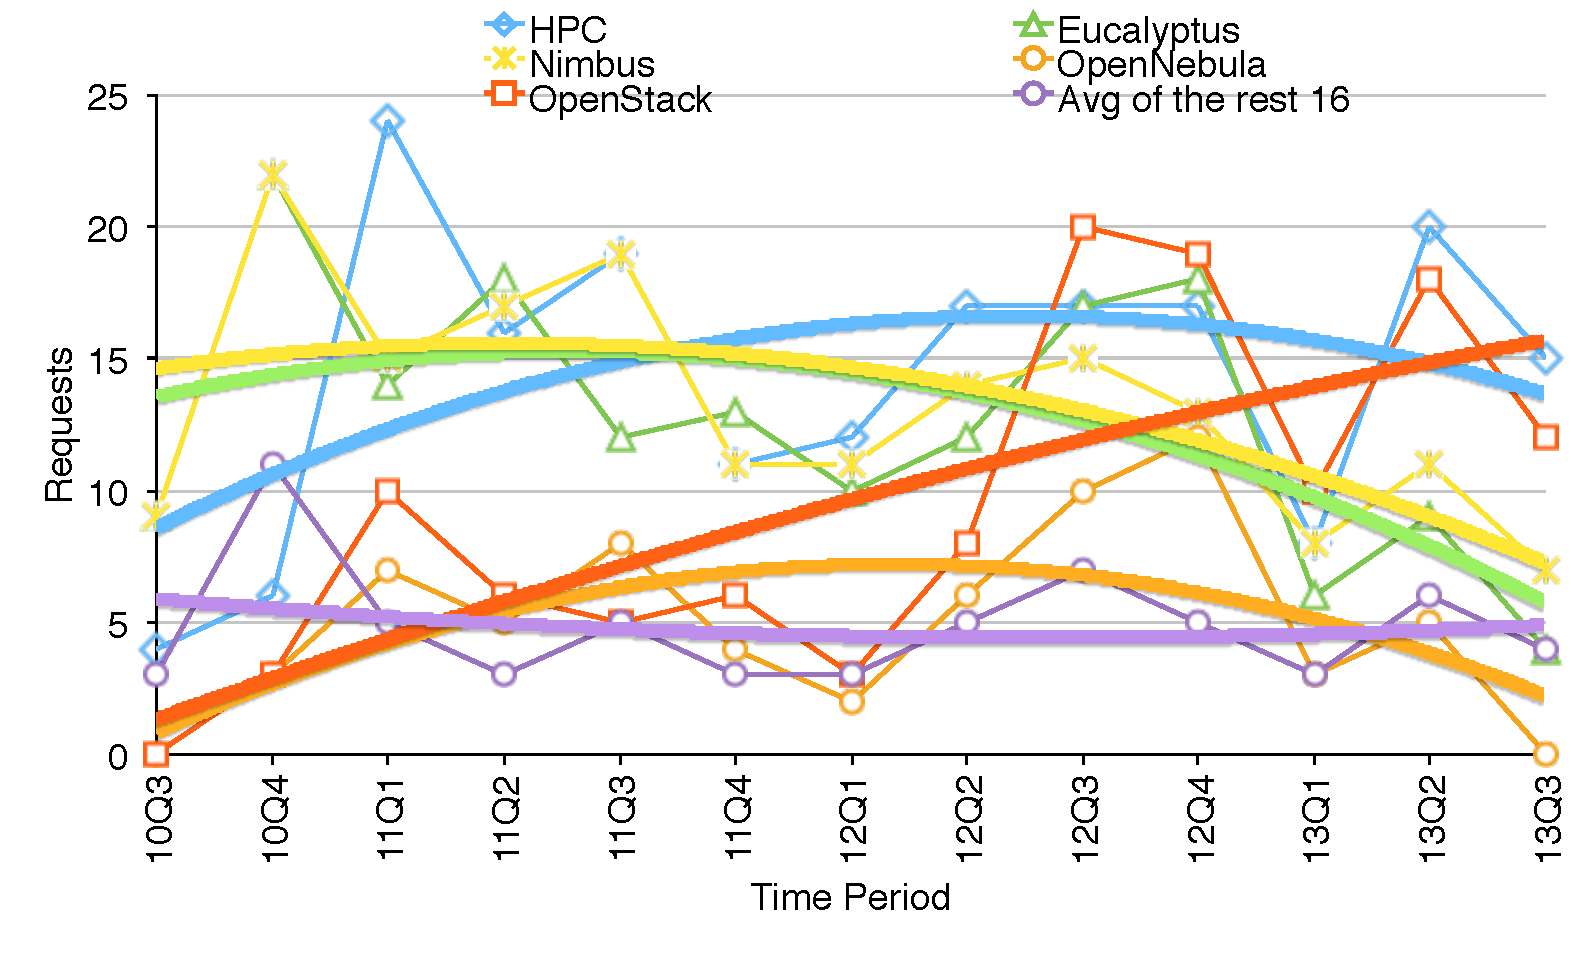
\includegraphics[width=1.0\textwidth]{images/trend-a.pdf}
  \caption{Requested technologies by project}\label{F:request-tech}
\end{figure}

From the overall project information we have also analysed the
frequency of the number of project members within the project and show
it in Figure~\ref{F:project-members}. Here we depict on the abscissa
classes of projects with varying members.  Assume we look at the
abscissa value of 10, This means that thease are all projects that
have project members between 10 and its previous category in this case
5. Hence, it will be all projects greater  5 and smaller or equal
10. With this calsssification  we see that the dominant unique number of
members within all projects is either one, two or thre members. Than
we have another class between 4 and 10 members, and the rest with more
than ten members. One of the projects had overall 186 registered
members, for an education class as part of a summer school. Looking at
the distribution of the members and associating them with reserach and
education projects, we find all projects with larger numbers of
projects to be education projects.


\begin{figure}[htb]
 \centering
    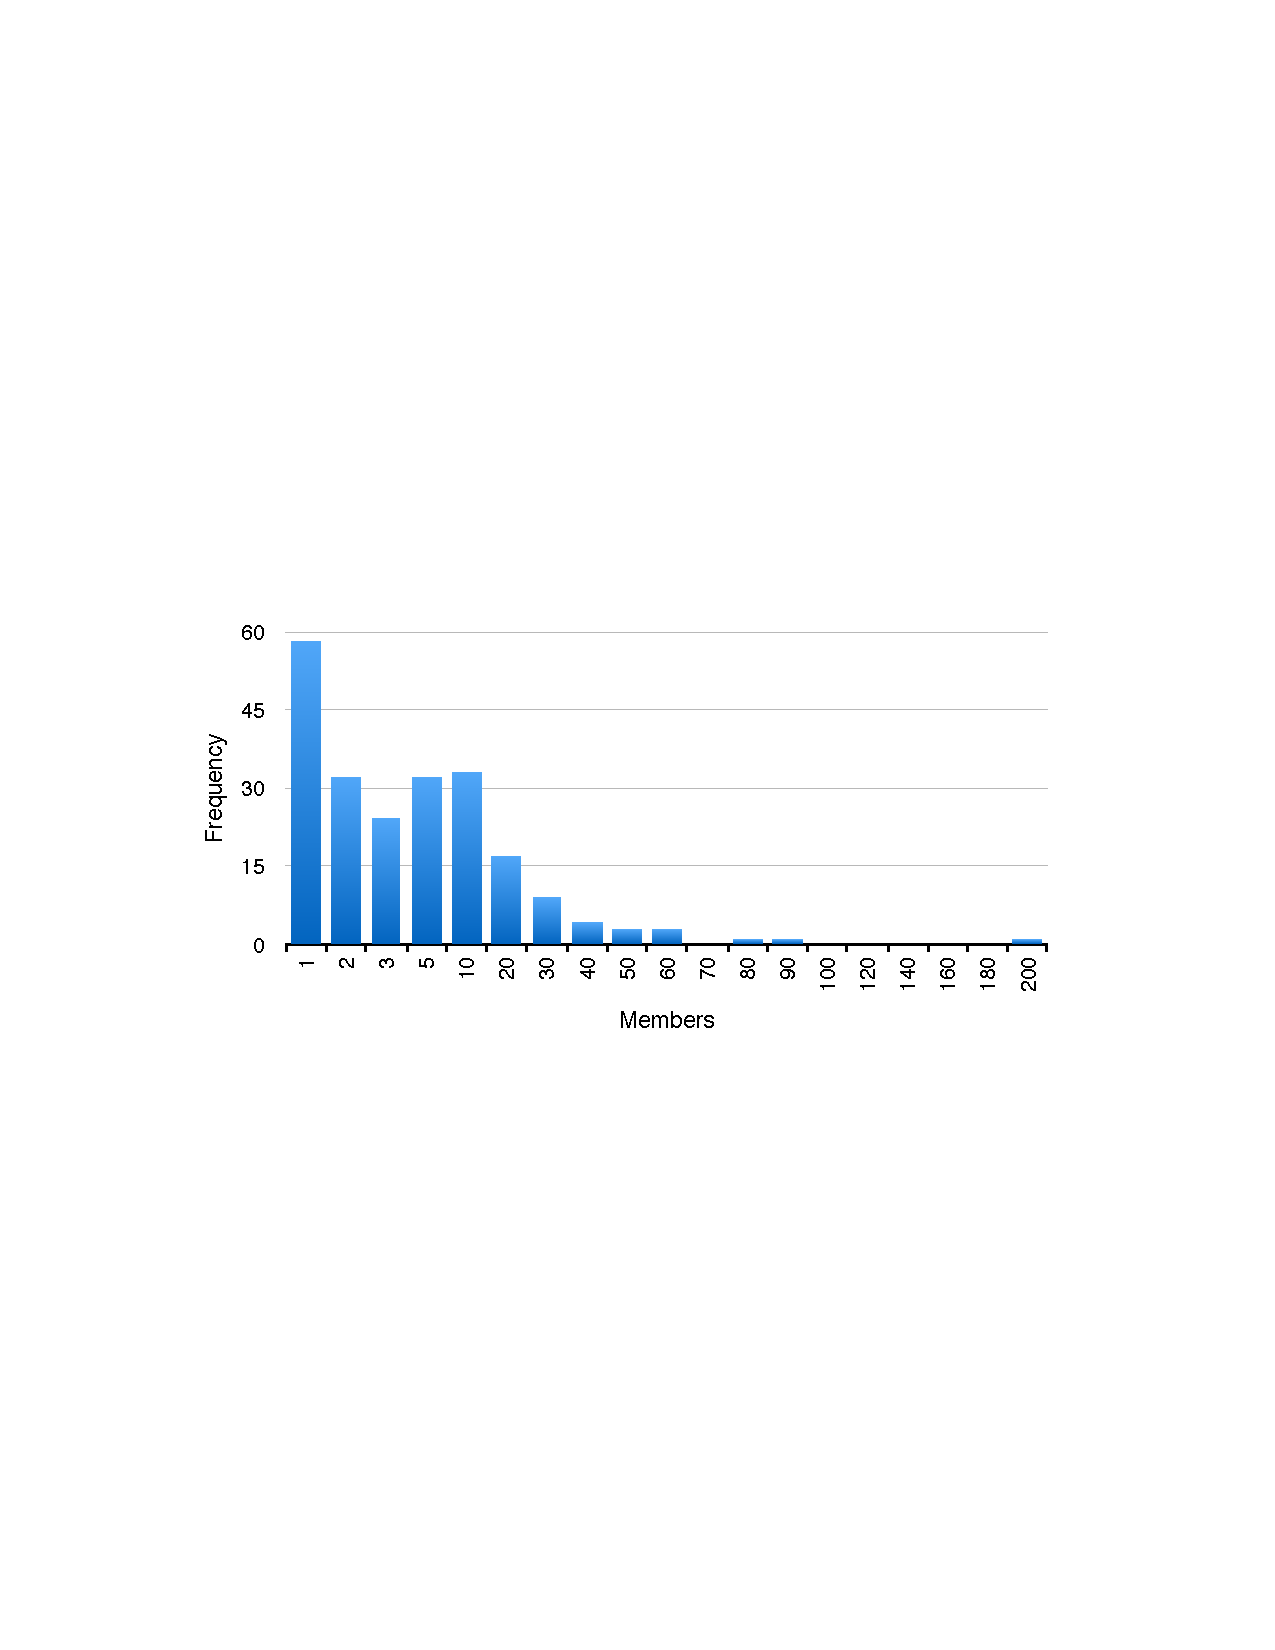
\includegraphics[width=1.0\textwidth]{images/project-frequency.pdf}
  \caption{Project Frequency.}\label{F:project-members}
\end{figure}

%Figure~\ref{F:bigdata-freq} shows the frequency distribution of technologies such as
%map/reduce, hadoop, and twister by year. In the chart we simply called
%the agglomoration of these technologies big data.  As we see relative
%to all projects requested within one year we identified a rising trend.

%\begin{figure}[htb]
%  \centering
%    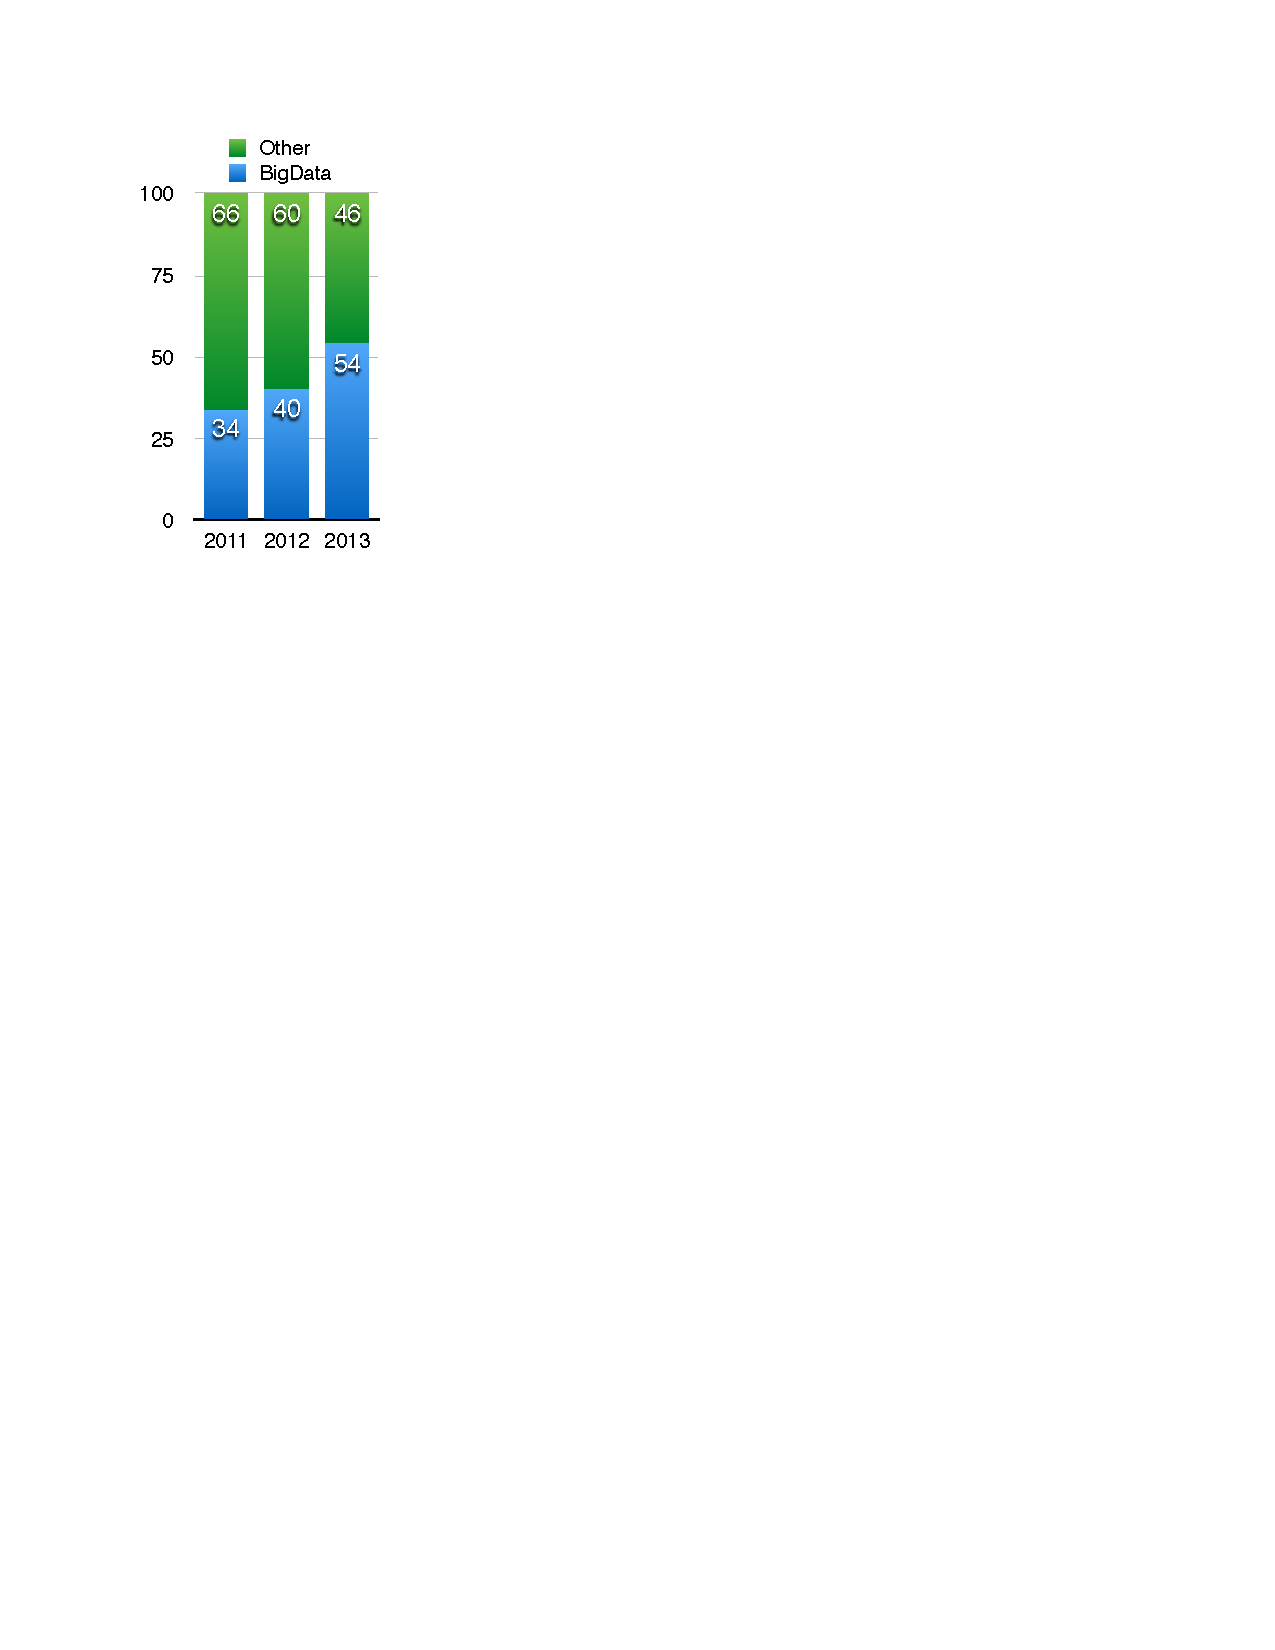
\includegraphics[width=0.2\textwidth]{images/bigdata-freq.pdf}
%  \caption{Big Data Project frequency.}\label{F:bigdata-freq}
%\end{figure}

Next we have taken from all projects in the categories as depicted in
\ref{F:freq-dis}. In contrast to XSEDE which provides a production HPC
system to the scientific community, the usage of FutureGrid is
dominated with 50\% by computer science related projects\footnote{is
  this for all projects or just within hadoop? This is not cear from
  the data I received.} Education is the next highest with 19\%.

\begin{figure}[htb]
  \centering
    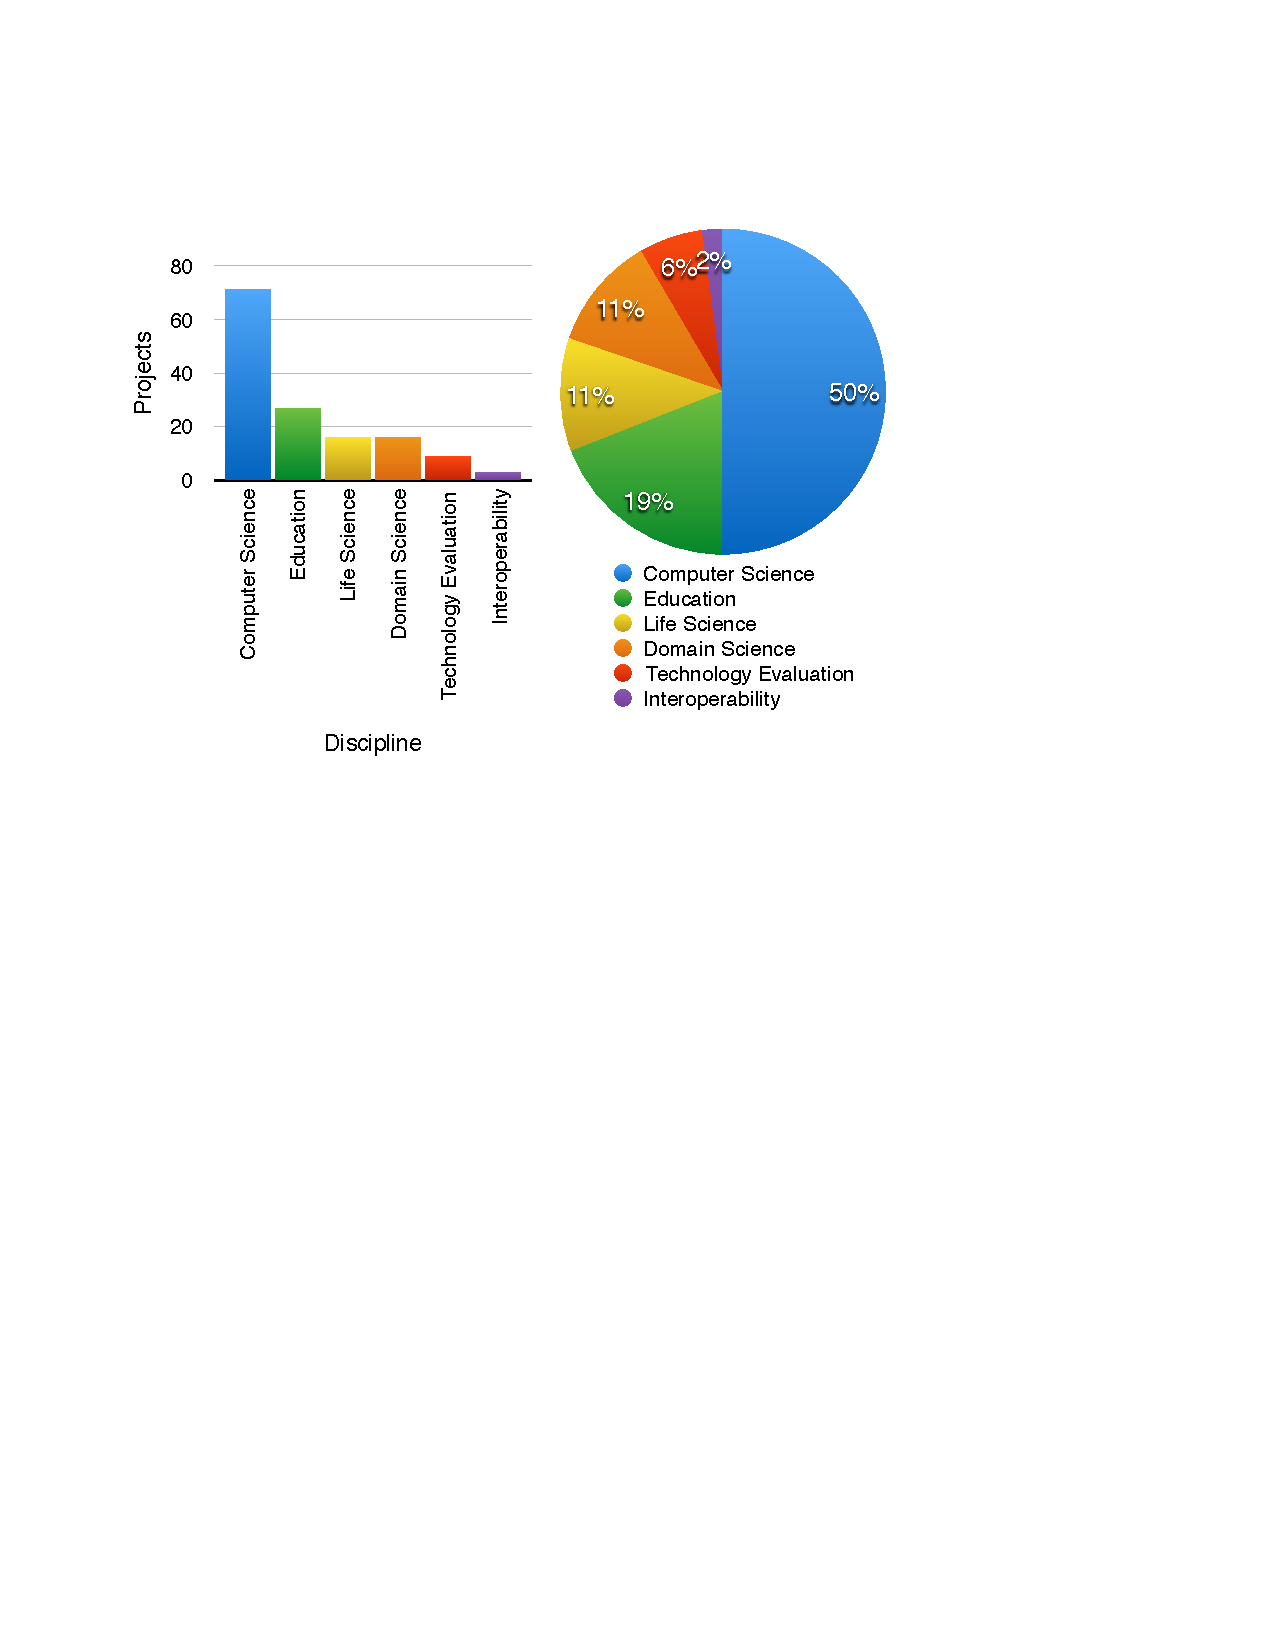
\includegraphics[width=1.0\textwidth]{images/project-disciplines.pdf}
  \caption{project disciplines.}
  \label{F:freq-dis}
\end{figure}

If we look at further into this data 

\begin{figure}[htb]
  \centering
    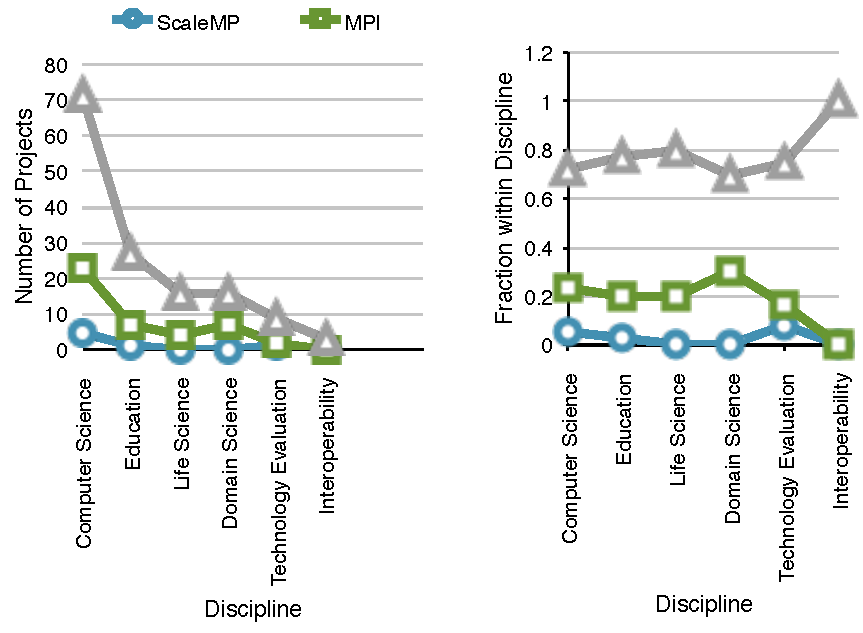
\includegraphics[width=1.0\textwidth]{images/trend-b.pdf}
  \caption{Requests by of technologies by discipline within a
    project. $\bigtriangleup$ = Map Reduce, Hadoop, or Twister,
    $\Box$\footnote{slash box does not show up, do we need another
      latex package}
  = MPI, $\circ$ = ScaleMP}
\end{figure}



\begin{figure}[htb]
  \centering
    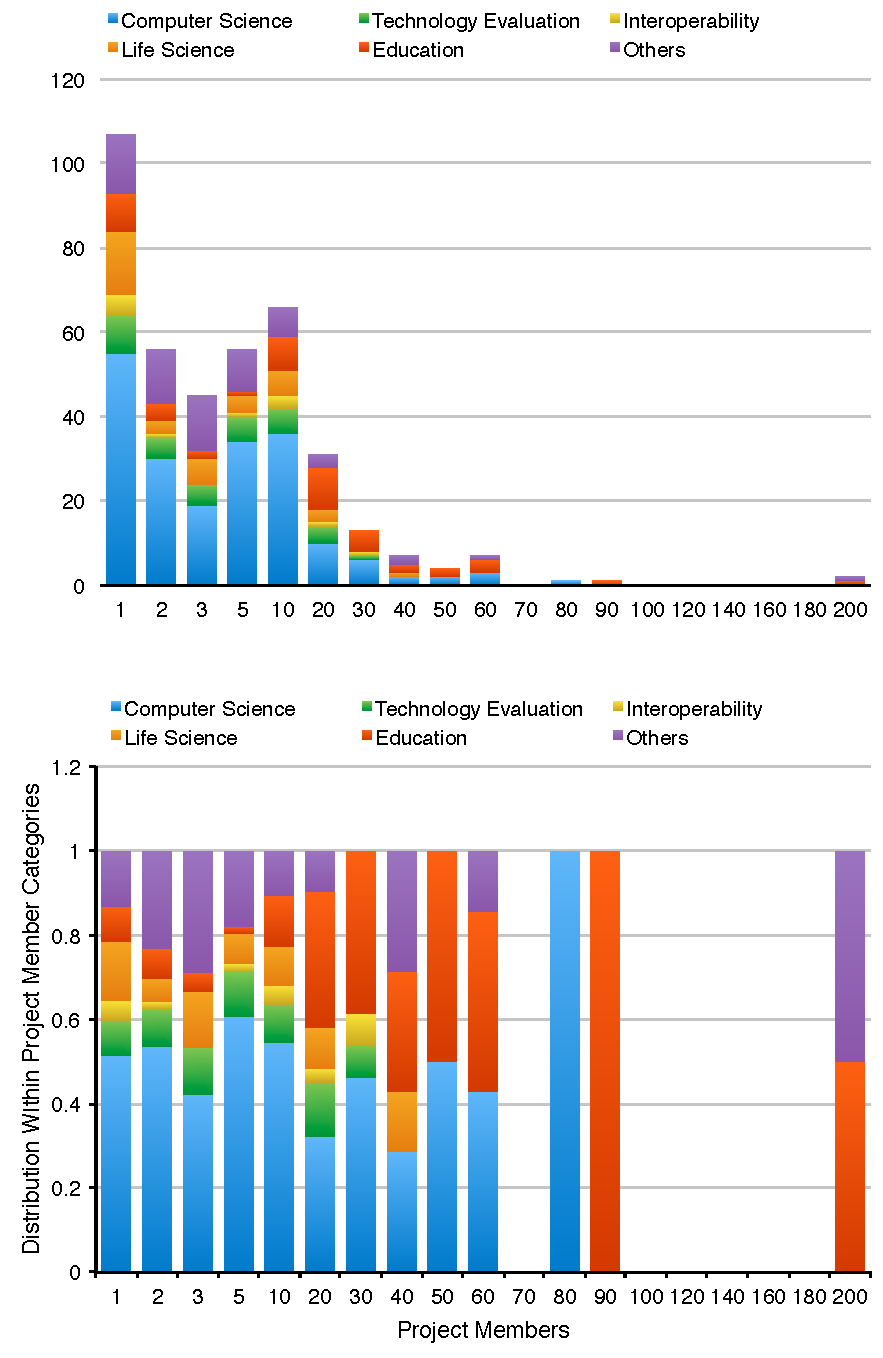
\includegraphics[width=1.0\textwidth]{images/project-member-dist.pdf}
  \caption{Project Member Dist.}
\end{figure}

\afterpage{\clearpage}